\documentclass[12pt]{book}
\usepackage[utf8]{inputenc}
\usepackage[spanish]{babel}
\usepackage{listings}
\usepackage{graphicx}

\begin{document}

\section{Singleton}

\subsection{Problema}

Durante el proceso de diseño de un sistema se requiere planificar el comportamiento de sus componentes, normalmente pueden surgir necesidades específicas para estos componentes, por ejemplo que una clase de la cual sólo debe existir una única instancia. Esta clase típicamente guarda información global para todo el sistema y esta información no debe ser inconsistente. Por esta razón se busca que la clase tenga únicamente una instancia, para sea un punto de acceso global, concentrado y seguro tanto para la lectura de datos como para la escritura.


\subsubsection{Ejemplos}

\begin{itemize}
    \item Archivo de configuración (bolsas de propiedades).
    \item Canales de comunicación (por ejemplo JNDI).
    \item Administradores de conexión con un DBMS.
\end{itemize}

\subsection{Intención}

El patrón previene la creación de múltiples instancias adicionales. Es común que una primera instancia sea creada al momento en que el sistema se inicializa, aunque esto puede diferir según la implementación del patrón. En los ejemplos mostrados más adelante la primera instancia se crea en el momento que el usuario haga el primer uso del objeto.
El patrón utiliza accesos estáticos para que los otros módulos se comuniquen con la única instancia del objeto de manera que sirve como un punto de acceso global a la información.


\newpage
\subsection{Solución}

Se implementa una clase que contiene una referencia estática a sí misma. Esta referencia típicamente es privada, y se accede por medio de métodos estáticos que encapsulan los llamados a la implementación. \\

\begin{figure}[h]
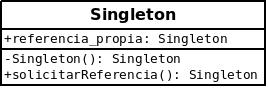
\includegraphics[width=8cm]{imagenes/singleton.jpeg}
\end{figure}


% Singleton tiene la peculiaridad que tiene varias implementaciones alternativas, la clásica, la ingenua y la segura 
\textbf{Implementación clásica:} \\
Para implementar un singleton se requiere quitar al usuario la capacidad de crear nuevas instancias de un objeto, por lo que la primera característica de esta implementación es crear un constructor privado.
Ya que se elimina la capacidad de construir objetos es necesario un método público que verifique si ya existe una instancia del mismo, en caso de existir previamente una instancia esta se retorna o en caso contrario se crea la instancia del objeto en cuestión.
Para que esto sea posible es necesario que el objeto tenga una referencia a su propia instancia, para que pueda ser retornada al ser consultada desde cualquier parte del sistema.

Como se puede apreciar en el código de ejemplo de esta implementación se desea un objeto que almacene el registro de jugadores, donde cada uno tendrá un identificador y este debe ser el mismo para todo el sistema.
Se puede apreciar como el constructor de la clase es privado, pero se puede crear a través del método solicitarReferencia() de manera que la referencia a la instancia se retornará a cualquier módulo que requiera información de este registro.

\begin{verbatim}
public class Registro {
	
    private static Registro puntero = null;
    
    private ArrayList<Integer> id_jugadores;
    
    private Registro() {
        id_jugadores = new ArrayList<Integer>();
    }
    
    public void agregarJugador(int id) {
        id_jugadores.add(id);
    }
    
    public ArrayList<Integer> getId_jugadores() {
        return id_jugadores;
    }
    
    public void mostarJugadores() {
        System.out.println(id_jugadores.toString());
    }
    
    public static Registro solicitarReferencia() {

        if (puntero == null) {
            puntero = new Registro();
        }   
        return puntero;
    }
}
\end{verbatim}

\textbf{Implementación ingenua:} \\
La implementación ingenua de un singleton se da cuando se crea un clase estática. Por naturaleza los métodos de este tipo de objeto pueden ser utilizados sin la necesidad de crear una instancia del objeto, por lo que sólo se crea una instancia en el sistema y no es responsabilidad del usuario crearla.
Este tipo de comportamiento es equivalente al de una biblioteca, se pueden usar los métodos que brinda, pero no se requiere tener una instancia de la clase para poder usarlos.

\begin{verbatim}
public class Matemática {
	
    public int mcd (int a, int b) {
        if (b == 0) {
            return a;
        }
        else {
            return mcd(b, a % b);
        }
    }
    
    public int mcm (int a, int b) {
        return (a * b) / mcd(a, b);
    }
}
\end{verbatim}

\newpage

\textbf{Caso de prueba:} \\
El código a continuación es un ejemplo de cómo se comporta el singleton. 
Se generan dos referencias hacia un objeto y se hacen inserciones de datos en el mismo. Normalmente un programa que no usa este patrón realizaría dos instancias del objeto y los datos querían separados, sin embargo gracias al patrón ambas referencias contienen la misma instancia del objeto, por lo que al mostrar los jugadores insertados en cada referencia se obtiene el mismo resultado, ya que se insertó sobre el mismo objeto.


\begin{verbatim}
public class Marcador {
    public static void main(String[] args) {
    
        Registro jugadores = Registro.solicitarReferencia();
    
        jugadores.agrgarJugador(1);
        jugadores.agrgarJugador(2);
    
        Registro copia_jugadores = Registro.solicitarReferencia();
    
        copia_jugadores.agrgarJugador(3);
        copia_jugadores.agrgarJugador(4);
        
        jugadores.mostarJugadores();
        copia_jugadores.mostarJugadores();	
    }
}
\end{verbatim}


\subsection{Opcional: Antipatrón}
Descripción breve de cómo el patrón puede ocasionar más problemas que soluciones. Por ejemplo la implementación segura de Singleton típicamente funciona como un antipatrón, generando problemas de rendimiento al requerir demasiadas verificaciones o sincronización innecesarias.

Esto no significa que la implementación segura de Singleton sea un antipatrón, como todo en patrones, depende de la naturaleza del problema. Más que nada prevenir una implementación inadecuada del patrón.
\end{document}
